\documentclass[11pt]{article}

\usepackage{amsmath,amssymb}
\usepackage{geometry}
\usepackage{graphicx}
\geometry{margin=1in}

\title{Inverse Hyperoperators and Information Storage}
\author{Thomas Bradley}
\date{\today}

\begin{document}
\maketitle

\section{Motivation}

Classical number-system extensions can be viewed through inverse operations:
\[
\mathbb{N} \xrightarrow{\text{subtraction}} \mathbb{Z}, \quad
\mathbb{Z} \xrightarrow{\text{division}} \mathbb{Q}, \quad
\mathbb{R} \xrightarrow{\text{roots/log}} \mathbb{C}.
\]
In each case, inverse maps require information that the prior space cannot always
store globally or continuously.

\section{Inverse-Information Principle}

Let $f$ be an operator and consider the inverse relation $f(x)=y$.
When inverse continuation introduces discrete branch parameters
\[
(b_1,\dots,b_r) \in \mathbb{Z}^r,
\]
we interpret these as independent information channels.

\medskip
\noindent\textbf{Conjecture (Inverse Hyperoperator Information Conjecture).}
If the inverse of $f$ requires $r$ independent branch parameters, then any
globally continuous representation requires at least $r$ extra real coordinates
beyond the base value coordinates.

\medskip
For complex-valued outputs (2 real coordinates), this predicts a minimal real
dimension
\[
2 + r.
\]

\section{Test Case: Inverse of $z^z$}

Consider
\[
w = z^z = e^{z\log z}.
\]
The inversion mixes multivalued logarithm branches and Lambert-$W$ branches,
suggesting two branch indices in practical continuation:
\[
k \in \mathbb{Z}, \qquad m \in \mathbb{Z}.
\]
Hence $r=2$, and the conjectured minimum is dimension $2+2=4$.

\section{Computational Results}

\subsection{Experiment 1: Single-loop baseline}
Using \texttt{../computational-gap-detection/01\_demo\_inverse\_z\_to\_z.py} on
\[
w(t)=0.01+2e^{it}, \quad t\in[0,2\pi],
\]
the tracked inverse path in $\mathbb{C}$ has nonzero endpoint gap:
\begin{itemize}
    \item Complex closure gap: \texttt{3.147208e+00}
    \item Lift span in $k$: \texttt{1.000000}
    \item Lift span in $m$: \texttt{0.223252}
\end{itemize}
This indicates branch accumulation not representable by a single complex branch over the loop.

\subsection{Experiment 2: Two-loop monodromy test}
Using \texttt{../computational-gap-detection/02\_path\_completion\_lift.py}, we test:
\begin{itemize}
    \item Loop A around $w^\ast=e^{-1/e}$: gap in $\mathbb{C}$ is \texttt{1.096153}
    \item Loop B around $0$: gap in $\mathbb{C}$ is \texttt{3.147208}
\end{itemize}
Lift-coordinate displacements are:
\begin{itemize}
    \item Loop A: $\Delta k_{\mathrm{lift}}\approx 0$, $\Delta m_{\mathrm{lift}}=1.000$
    \item Loop B: $\Delta k_{\mathrm{lift}}=1.000$, $\Delta m_{\mathrm{lift}}=0.223$
\end{itemize}
So the two loops excite different branch-information channels.

\section{How the Data Relates to the Conjecture}

The data supports the following interpretation:
\begin{itemize}
    \item Closed loops in the $w$-plane need not produce closed tracked inverse paths in $\mathbb{C}$.
    \item Additional lift coordinates vary continuously and record sheet change.
    \item For inverse $z^z$, two independent branch effects appear, matching the $r=2$ hypothesis and motivating a four-real-dimensional state description.
\end{itemize}

\section{What This Does Not Prove}

These scripts provide computational evidence, not a formal proof.
In particular, they do \emph{not} prove algebraic closure of an inverse map in quaternion arithmetic.
They demonstrate continuity of a lifted coordinate model and nontrivial monodromy in $\mathbb{C}$.

\section{Limitations and Next Steps}

\begin{itemize}
    \item Nearest-neighbour continuation is heuristic and path dependent.
    \item Results should be stress-tested across radii, centers, and discretization density.
    \item A proof-level treatment likely needs covering-space/monodromy formalism.
\end{itemize}

\begin{figure}[h]
    \centering
    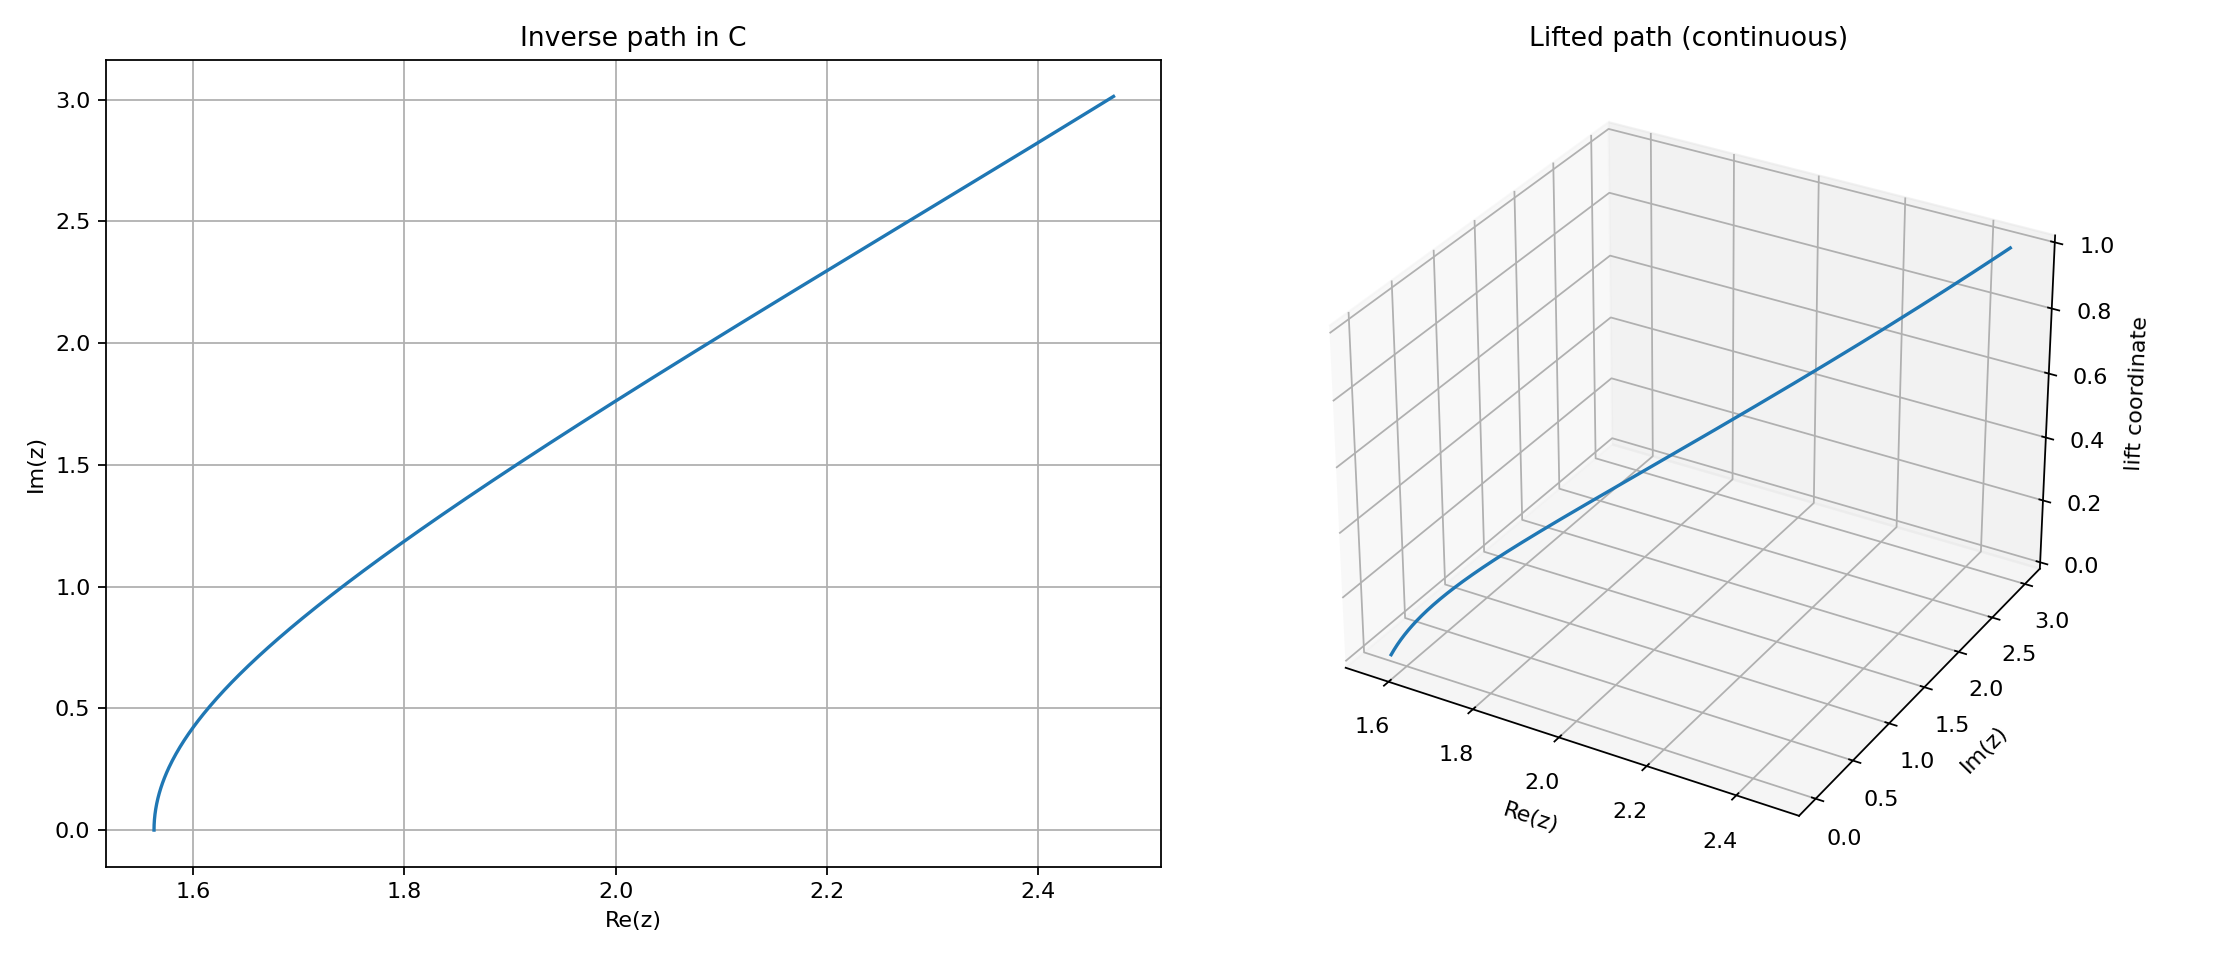
\includegraphics[width=0.92\textwidth]{../computational-gap-detection/inverse_z_to_z_demo.png}
    \caption{Experiment 1: baseline loop. Left: tracked inverse path in $\mathbb{C}$. Right: lifted-coordinate view.}
\end{figure}

\begin{figure}[h]
    \centering
    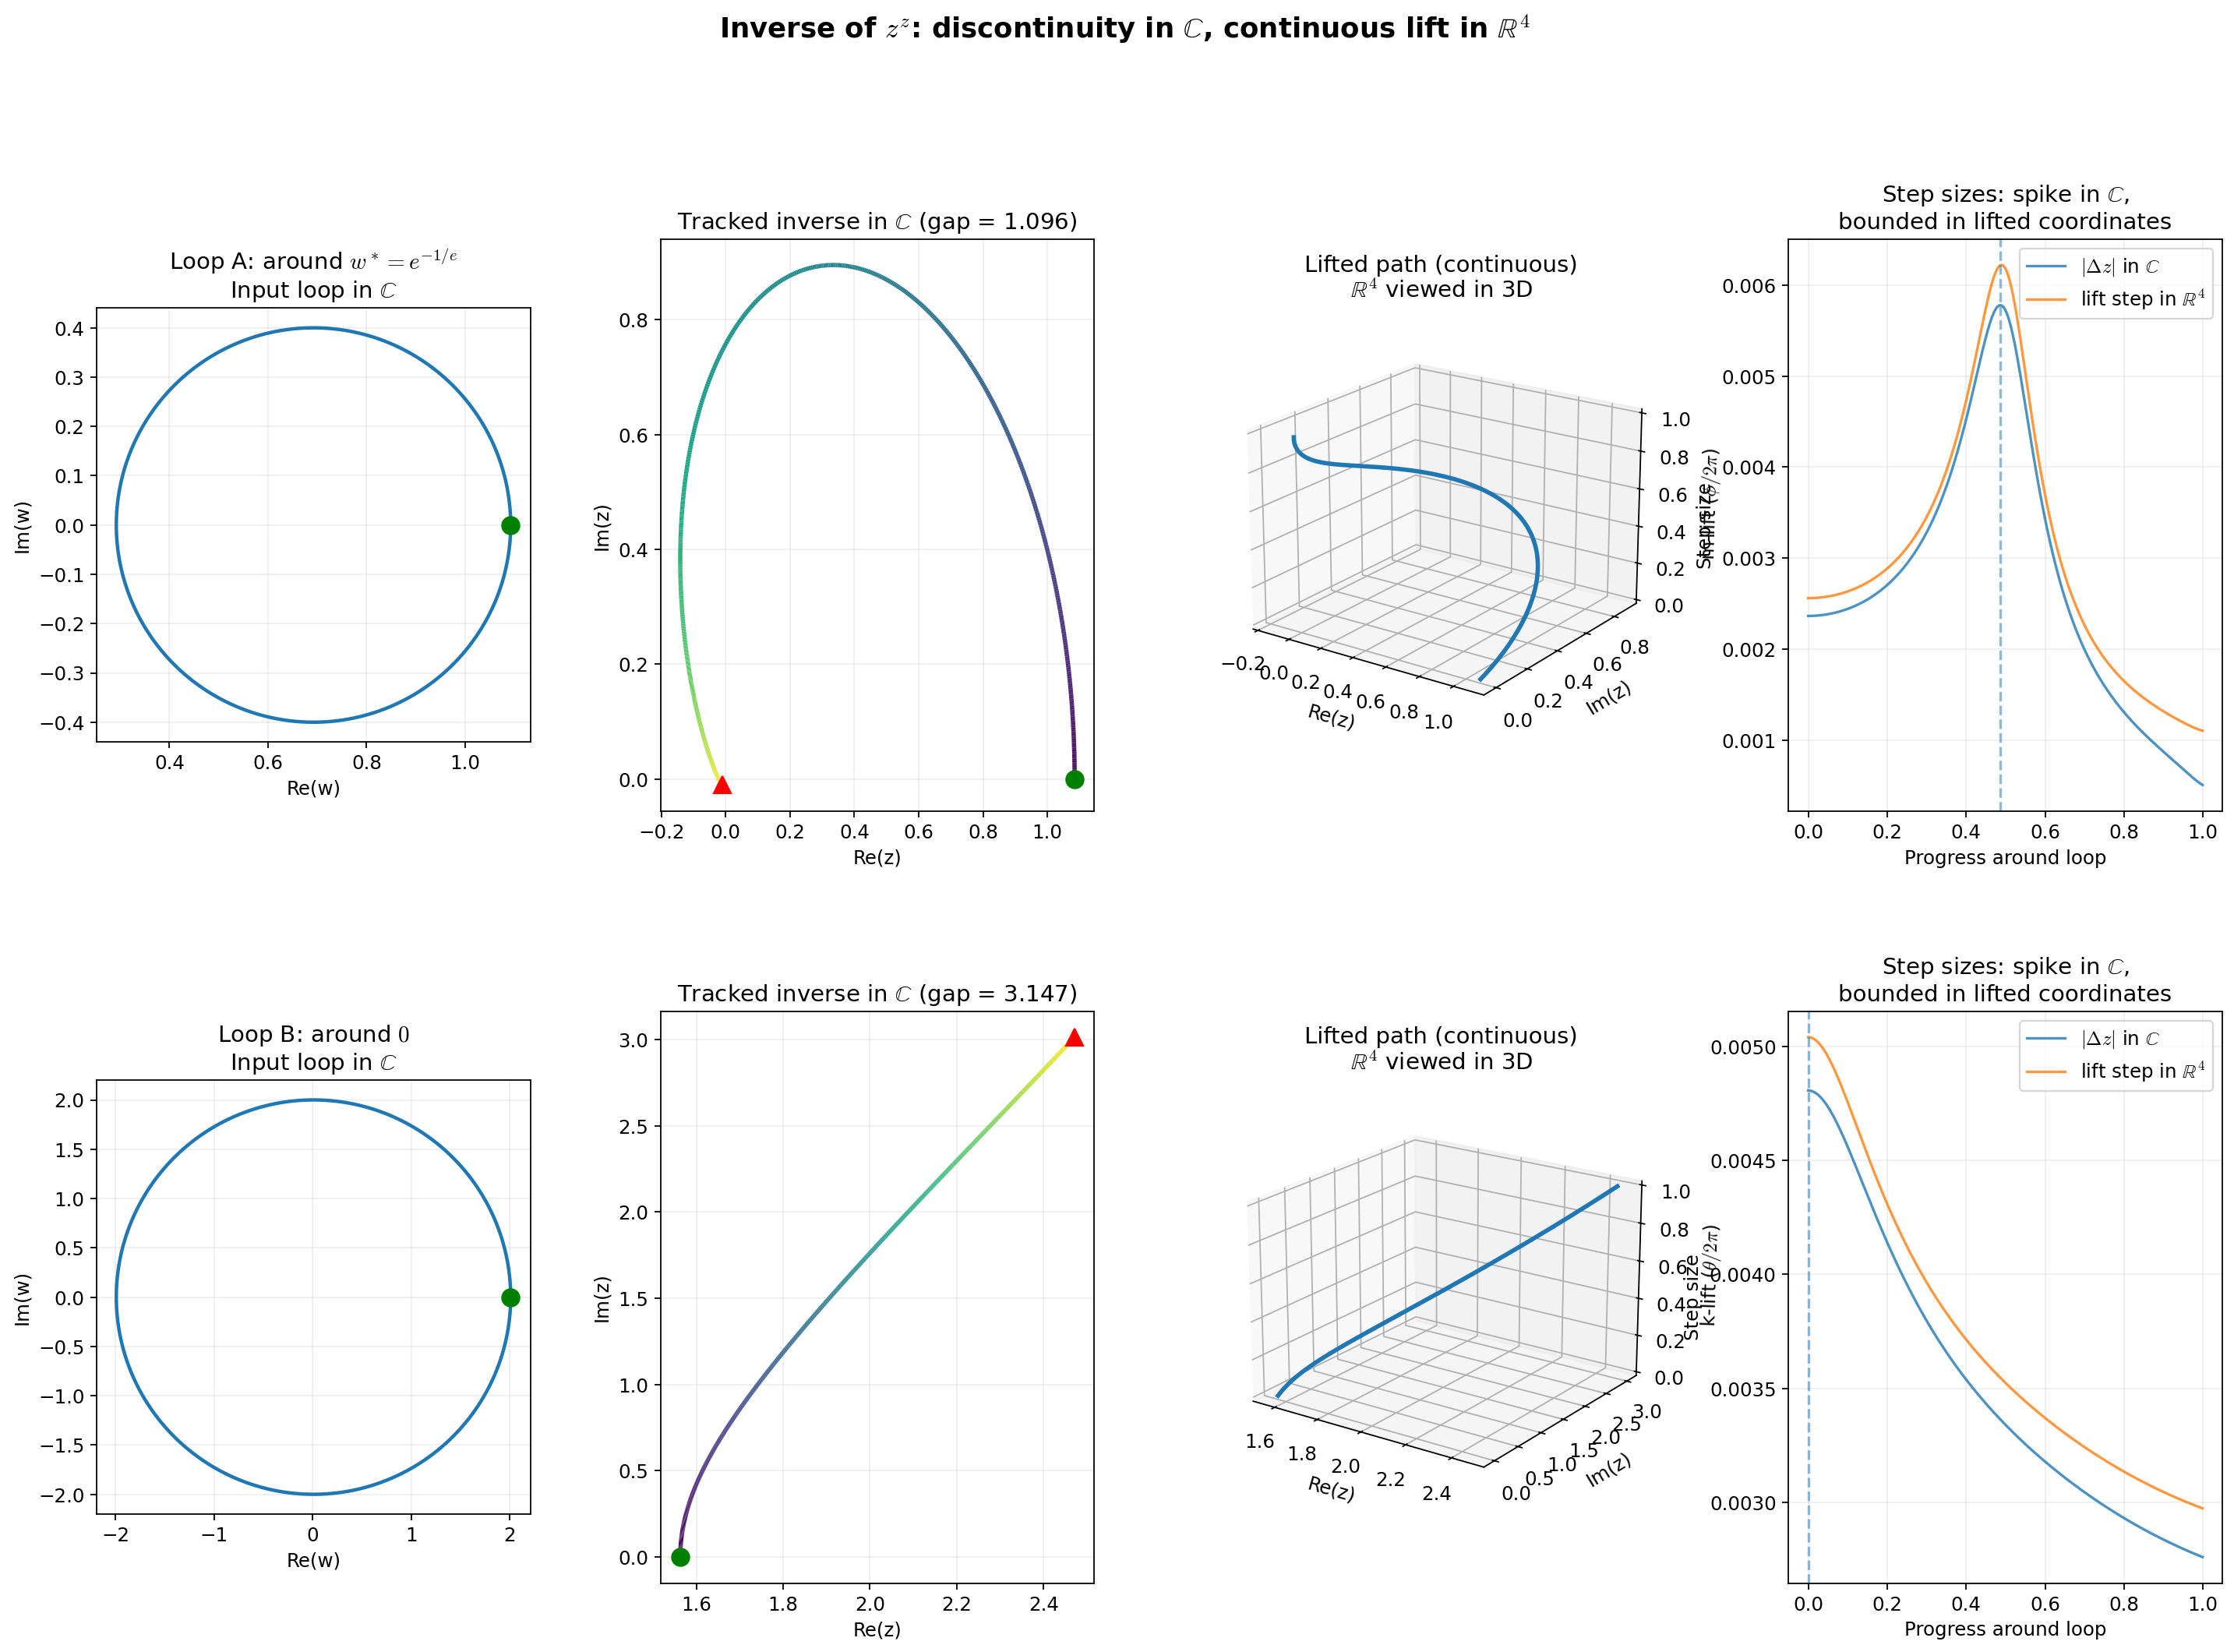
\includegraphics[width=0.98\textwidth]{../computational-gap-detection/fig_path_completion_lift.png}
    \caption{Experiment 2: two-loop comparison around $w^\ast$ and $0$, showing complex gaps and lift diagnostics.}
\end{figure}

\end{document}
